\documentclass{tietreport}

% Import images
\usepackage{graphicx}
\usepackage{booktabs}
\usepackage{longtable}
\usepackage{array}
\usepackage{float}
\usepackage{placeins}
\usepackage{rotating}

% Bibliography configuration
\usepackage[
  date=year,
  style=alphabetic,
  backend=biber,
  sorting=nty,
  maxnames=5,
  minnames=3,
  maxalphanames=4,
  minalphanames=3,
  backref=true,
  doi=false,
  isbn=false,
  url=false,
  eprint=false
]{biblatex}
\addbibresource{references.bib}

% Give TeX room to resolve awkward lines containing long
% typewriter identifiers rather than overflowing the margin.
\setlength{\emergencystretch}{3em}
% Keep floats inside the section that refers to them.
\let\oldsection\section
\renewcommand{\section}{\FloatBarrier\oldsection}

%% ==================================================
%% CUSTOMIZE THESE FIELDS FOR YOUR PROJECT
%% ==================================================

% Course/Lab header
\TitlePageHeader{%
  UCS 503 Software Engineering Project Report%
}

% Main project title
\ProjectTitle{%
  CampusCycle%
}

% Subtitle or project description
\ProjectSubTitle{%
  Smart Campus Bicycle Sharing and
  Mobility Management System%
}

% Student information
\author{%
  \texttt{102XXXXXXX} Guneet Singh Nagi \\
  \texttt{102XXXXXXX} Prabhnoor Oberoi%
}

% Group number, degree, year, program
\TitlePageSubText{%
  Group: \texttt{XXXX} BE Third Year, CSE%
}

% Faculty advisor/guide name
\AdvisorName{%
  Dr. Faculty Member Name%
}

% Evaluation period and department info
\TitlePageFooterText{{%
    \large Mid-Semester Evaluation \\[0.2cm]
    \bfseries Computer Science and Engineering
    Department%
  } \\[0.15cm]
  Thapar Institute of Engineering and Technology,
  Patiala%
}

%% ==================================================

\begin{document}

% Generate title page
\maketitle

% Table of contents (auto-generated from chapters)
\tableofcontents

% ===== CHAPTER 1: INTRODUCTION =====

\chapter{Introduction}

\section{Background and Context}

A university campus is large enough that walking
between a hostel, an academic block, the library and
the sports complex consumes a noticeable part of a
student's day, yet far too small for motorised
transport to be worthwhile. This is the classic
last-mile problem, and shared bicycles are a
well-established answer to it: public bike-sharing
schemes have been deployed in several hundred cities
worldwide, and the research literature consistently
identifies availability information and fleet
maintenance as the factors that decide whether such a
scheme is used or abandoned~\cite{shaheen2010,
fishman2016}.

A bicycle-sharing scheme, however, is not solved by
simply buying bicycles. Without a system behind them,
the fleet accumulates the familiar failures: cycles
pile up at one station while another stands empty, a
bicycle with failed brakes is rented out because
nobody recorded the fault, cycles leave the campus and
are not recovered, and the administration has no
evidence on which to base decisions about where cycles
should be placed.

CampusCycle addresses that gap. It is a web
application through which a student locates an
available bicycle, identifies it by scanning the QR
code printed on it, rides between docking stations and
returns it, while an administrator manages the fleet,
tracks every ride, processes reported faults and reads
usage analytics drawn from the live database.

\subsection{Problem Statement}

Design and build a centralised system for managing a
campus bicycle-sharing service that:

\begin{enumerate}
  \item tells a student, accurately and in real time,
    where a usable bicycle can be found;
  \item records every rental from start to finish so
    that a cycle is never in two places at once and a
    student never holds two cycles at once;
  \item ensures that a bicycle reported as unsafe
    cannot be rented out again until it has been
    inspected; and
  \item gives the administration figures about fleet
    utilisation, station demand and maintenance load
    that are computed from the system's own records
    rather than estimated.
\end{enumerate}

The difficulty in such a system is not any single
feature. It is that several of these requirements are
\emph{invariants} rather than screens: statements that
must hold no matter which part of the application is
running, and no matter how many users act at the same
time. Much of the design work reported here is
concerned with where such invariants are enforced.

\section{Project Objectives}

The objectives below were set in the project proposal.
Each is stated with the criterion by which it is
judged, and the status at this evaluation.

\begin{enumerate}
  \item \textbf{Account management and role
    separation.} Students register and sign in; an
    administrator console is reachable only by an
    administrator account. \emph{Criterion:} every
    administrative endpoint rejects a student token.
    \emph{Status: complete.}

  \item \textbf{QR-based bicycle identification.} Each
    bicycle carries a unique QR code which the backend
    resolves to a bicycle record and its current
    state. \emph{Criterion:} an unknown code and an
    unavailable cycle are both refused, with distinct
    responses. \emph{Status: complete.}

  \item \textbf{Rental and return workflow.} A student
    starts a ride, sees it in progress and returns the
    cycle at an approved station. \emph{Criterion:}
    two students attempting the same cycle at the same
    instant produce exactly one rental.
    \emph{Status: complete.}

  \item \textbf{Interactive campus map.} Stations are
    shown on a map of the campus with their live
    availability. \emph{Criterion:} the map and the
    station list never disagree, because both derive
    availability from one rule.
    \emph{Status: complete.}

  \item \textbf{Complete rental records.} Every ride
    is retained and can be inspected by the student
    who took it and by an administrator.
    \emph{Criterion:} a student cannot read another
    student's ride, by any route.
    \emph{Status: complete.}

  \item \textbf{Fault reporting and maintenance
    management.} Students report faults; the
    administration works them through a defined
    lifecycle. \emph{Criterion:} a cycle with an
    unresolved safety fault cannot be rented or
    returned to service. \emph{Status: complete.}

  \item \textbf{Usage analytics.} The administration
    sees fleet, station and ridership figures over a
    selectable period. \emph{Criterion:} every figure
    is a database aggregate, and the page survives an
    empty database. \emph{Status: complete.}

  \item \textbf{Campus geofencing.} A configurable
    campus boundary, with violations recorded and
    surfaced for action. \emph{Criterion:} a repeated
    breach does not produce repeated alerts.
    \emph{Status: complete as a software
    demonstration; see Section~\ref{sec:geofence}
    for the limitation that matters.}

  \item \textbf{Demand prediction and redistribution.}
    Prediction of station-level demand from historical
    rentals, and redistribution advice derived from
    it. \emph{Status: deferred to the next phase}, for
    the reason given in Section~\ref{sec:scope}.
\end{enumerate}

\section{Scope of This Report}
\label{sec:scope}

Development was organised into phases. Phase~1 built
the core rental system: accounts and roles, stations,
the fleet, QR identification, the rental and return
workflow, and an administrative dashboard. Phase~2,
which this report covers in full, added the campus
map, station availability, ride history, maintenance
management, usage analytics and software geofencing.

The machine-learning demand-prediction module was
deliberately held back rather than attempted
alongside Phase~2. A demand model is only as good as
the ridership history it is trained on, and that
history is produced by the very modules Phase~2
delivers. Building the analytics layer first means the
model will be trained on recorded data with a known
schema rather than on synthetic figures. Both this
report and the system therefore describe a complete
two-phase implementation, with prediction scheduled
as the next phase.

% ===== CHAPTER 2: METHODOLOGY & DESIGN =====

\chapter{Methodology and Design}

\section{Development Approach}

The system was developed incrementally, in two phases
with a working, tested application at the end of each.
Phase~2 was implemented against the running Phase~1
system under three self-imposed constraints: the
Phase~1 database was to be migrated rather than
rebuilt, the existing architectural conventions were
to be reused rather than replaced, and the Phase~1
test suite was to keep passing unchanged. The last of
these functioned as a regression gate; the schema
constraint is why all Phase~2 schema changes are
additive and idempotent (Section~\ref{sec:migrations}).

\section{System Architecture}

\subsection{High-Level Design}

CampusCycle follows a three-tier architecture
(Figure~\ref{fig:arch}). The browser holds the entire
user interface; the Node.js process holds all business
rules; PostgreSQL holds all state. The two tiers
communicate only over a JSON REST API, which means the
server never produces markup and the browser never
issues a query.

\begin{figure}[htbp]
  \centering
  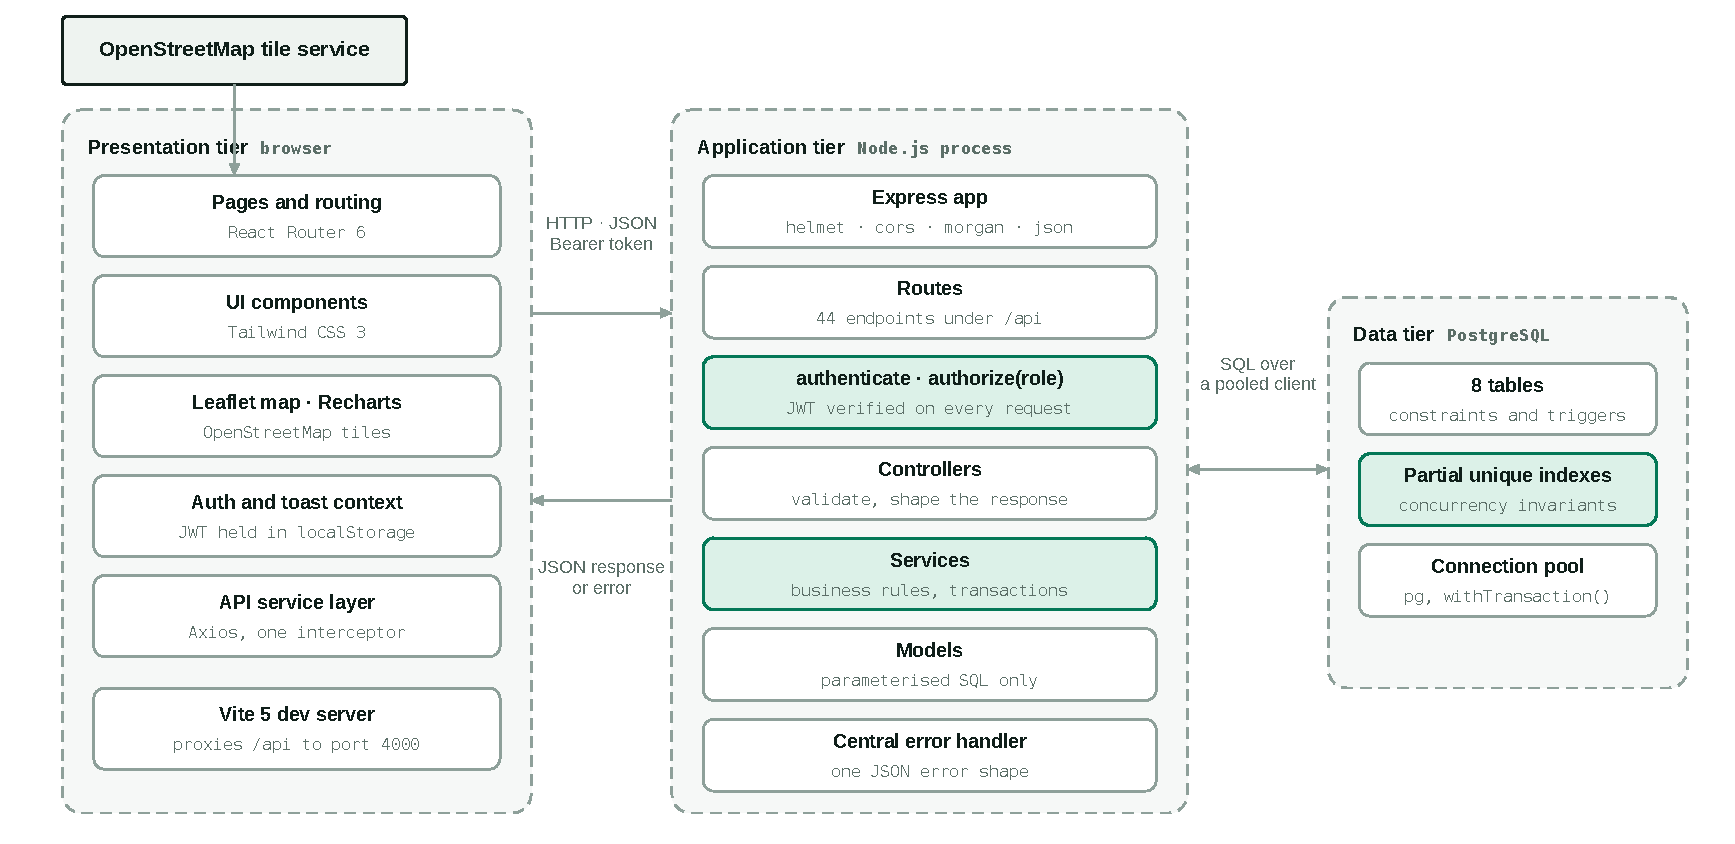
\includegraphics[width=\textwidth]{figures/arch.pdf}
  \caption{Three-tier architecture. Each request
    crosses the server layers in order, and only the
    model layer issues SQL.}
  \label{fig:arch}
\end{figure}

The application tier is deliberately layered, and a
request always crosses the layers in the same order:

\begin{itemize}
  \item \textbf{Routes} declare the URL, the HTTP verb
    and the roles permitted to reach the handler.
  \item \textbf{Middleware} verifies the JSON Web
    Token~\cite{rfc7519} and attaches the caller's
    identity and role to the request.
  \item \textbf{Controllers} read and validate request
    parameters and shape the response. They contain no
    business rules.
  \item \textbf{Services} hold the business rules, and
    own every database transaction.
  \item \textbf{Models} issue parameterised SQL and
    nothing else.
\end{itemize}

Keeping transactions in the service layer, rather than
in controllers or models, is what makes the
concurrency rules in Section~\ref{sec:concurrency}
expressible at all: a rule that spans two tables has
exactly one place it can live.

\subsection{Technical Stack}

\begin{table}[htbp]
\centering
\begin{tabular}{@{}lll@{}}
\toprule
\textbf{Layer} & \textbf{Technology} &
\textbf{Version} \\
\midrule
User interface   & React with Vite        & 18.3 / 5.4 \\
Styling          & Tailwind CSS           & 3.4 \\
Routing          & React Router           & 6.24 \\
HTTP client      & Axios                  & 1.7 \\
Mapping          & Leaflet + OpenStreetMap & 1.9.4 \\
Charts           & Recharts               & 2.15 \\
Server runtime   & Node.js                & $\geq 18$ \\
Web framework    & Express                & 4.19 \\
Database         & PostgreSQL             & $\geq 13$ \\
Database driver  & node-postgres (pg)     & 8.12 \\
Authentication   & jsonwebtoken, bcryptjs & 9.0 / 2.4 \\
HTTP hardening   & helmet, cors           & 7.1 / 2.8 \\
Version control  & Git and GitHub         & --- \\
\bottomrule
\end{tabular}
\caption{Implementation stack.}
\label{tab:stack}
\end{table}

\subsubsection*{Departure from the proposal:
PostgreSQL in place of MySQL}

The proposal named MySQL. The implementation uses
PostgreSQL, and the reason is specific rather than a
matter of preference. Three of the system's invariants
are enforced by \emph{partial unique
indexes}~\cite{pgindexes} --- unique indexes that
apply only to the rows matching a predicate:

\begin{itemize}
  \item at most one \texttt{ACTIVE} rental per
    student;
  \item at most one \texttt{ACTIVE} rental per
    bicycle;
  \item at most one unresolved geofence alert per
    bicycle.
\end{itemize}

MySQL has no partial indexes, so each of these rules
would have to be enforced in application code, where
it is subject to the race conditions discussed in
Section~\ref{sec:concurrency}. PostgreSQL also
supplies three features the analytics module relies
on: \texttt{FILTER} clauses on aggregates,
\texttt{generate\_series} for producing a continuous
date axis including days on which nothing happened,
and \texttt{JSONB} for storing the geofence polygon.
The cost of the change was confined to the schema
files and the database driver; no application logic
depends on the vendor.

\section{Data Flow}

The data-flow diagrams use Gane--Sarson
notation~\cite{demarco1979}. Figure~\ref{fig:dfd0}
fixes the system boundary, Figure~\ref{fig:dfd1}
decomposes the system into processes and stores, and
Figures~\ref{fig:dfd2m} and~\ref{fig:dfd2g} explode
the two processes whose internal behaviour is not
obvious from the level-1 view.

\begin{figure}[htbp]
  \centering
  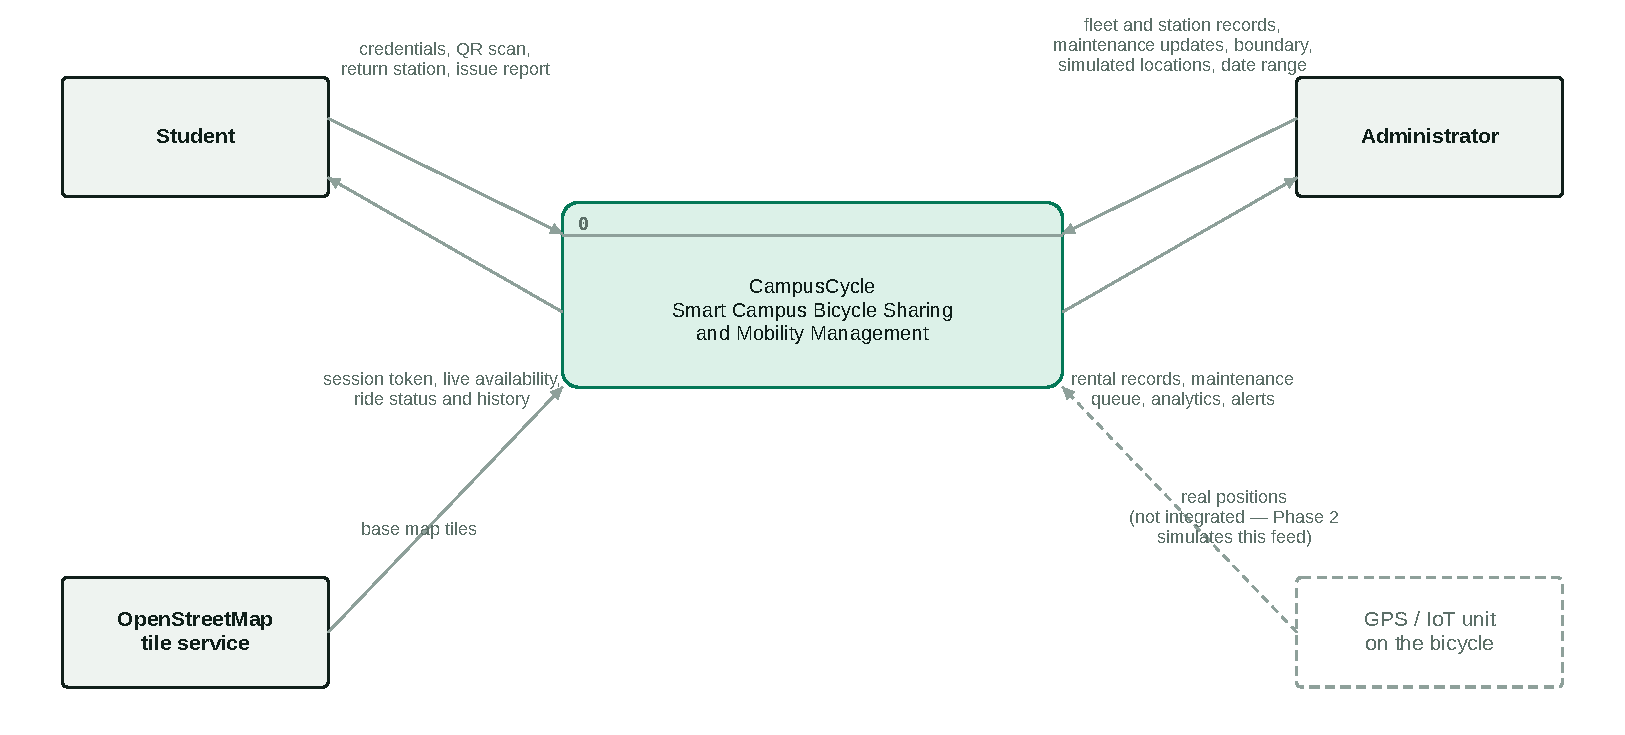
\includegraphics[width=\textwidth]{figures/dfd-l0.pdf}
  \caption{Context diagram. The dashed feed records an
    honest gap: the bicycles carry no GPS hardware, so
    every position the system holds was submitted by
    an administrator and stored as simulated.}
  \label{fig:dfd0}
\end{figure}

% Turned sideways on a page of its own: at portrait
% width the process labels would be too small to read
% in print.
\begin{sidewaysfigure}
  \centering
  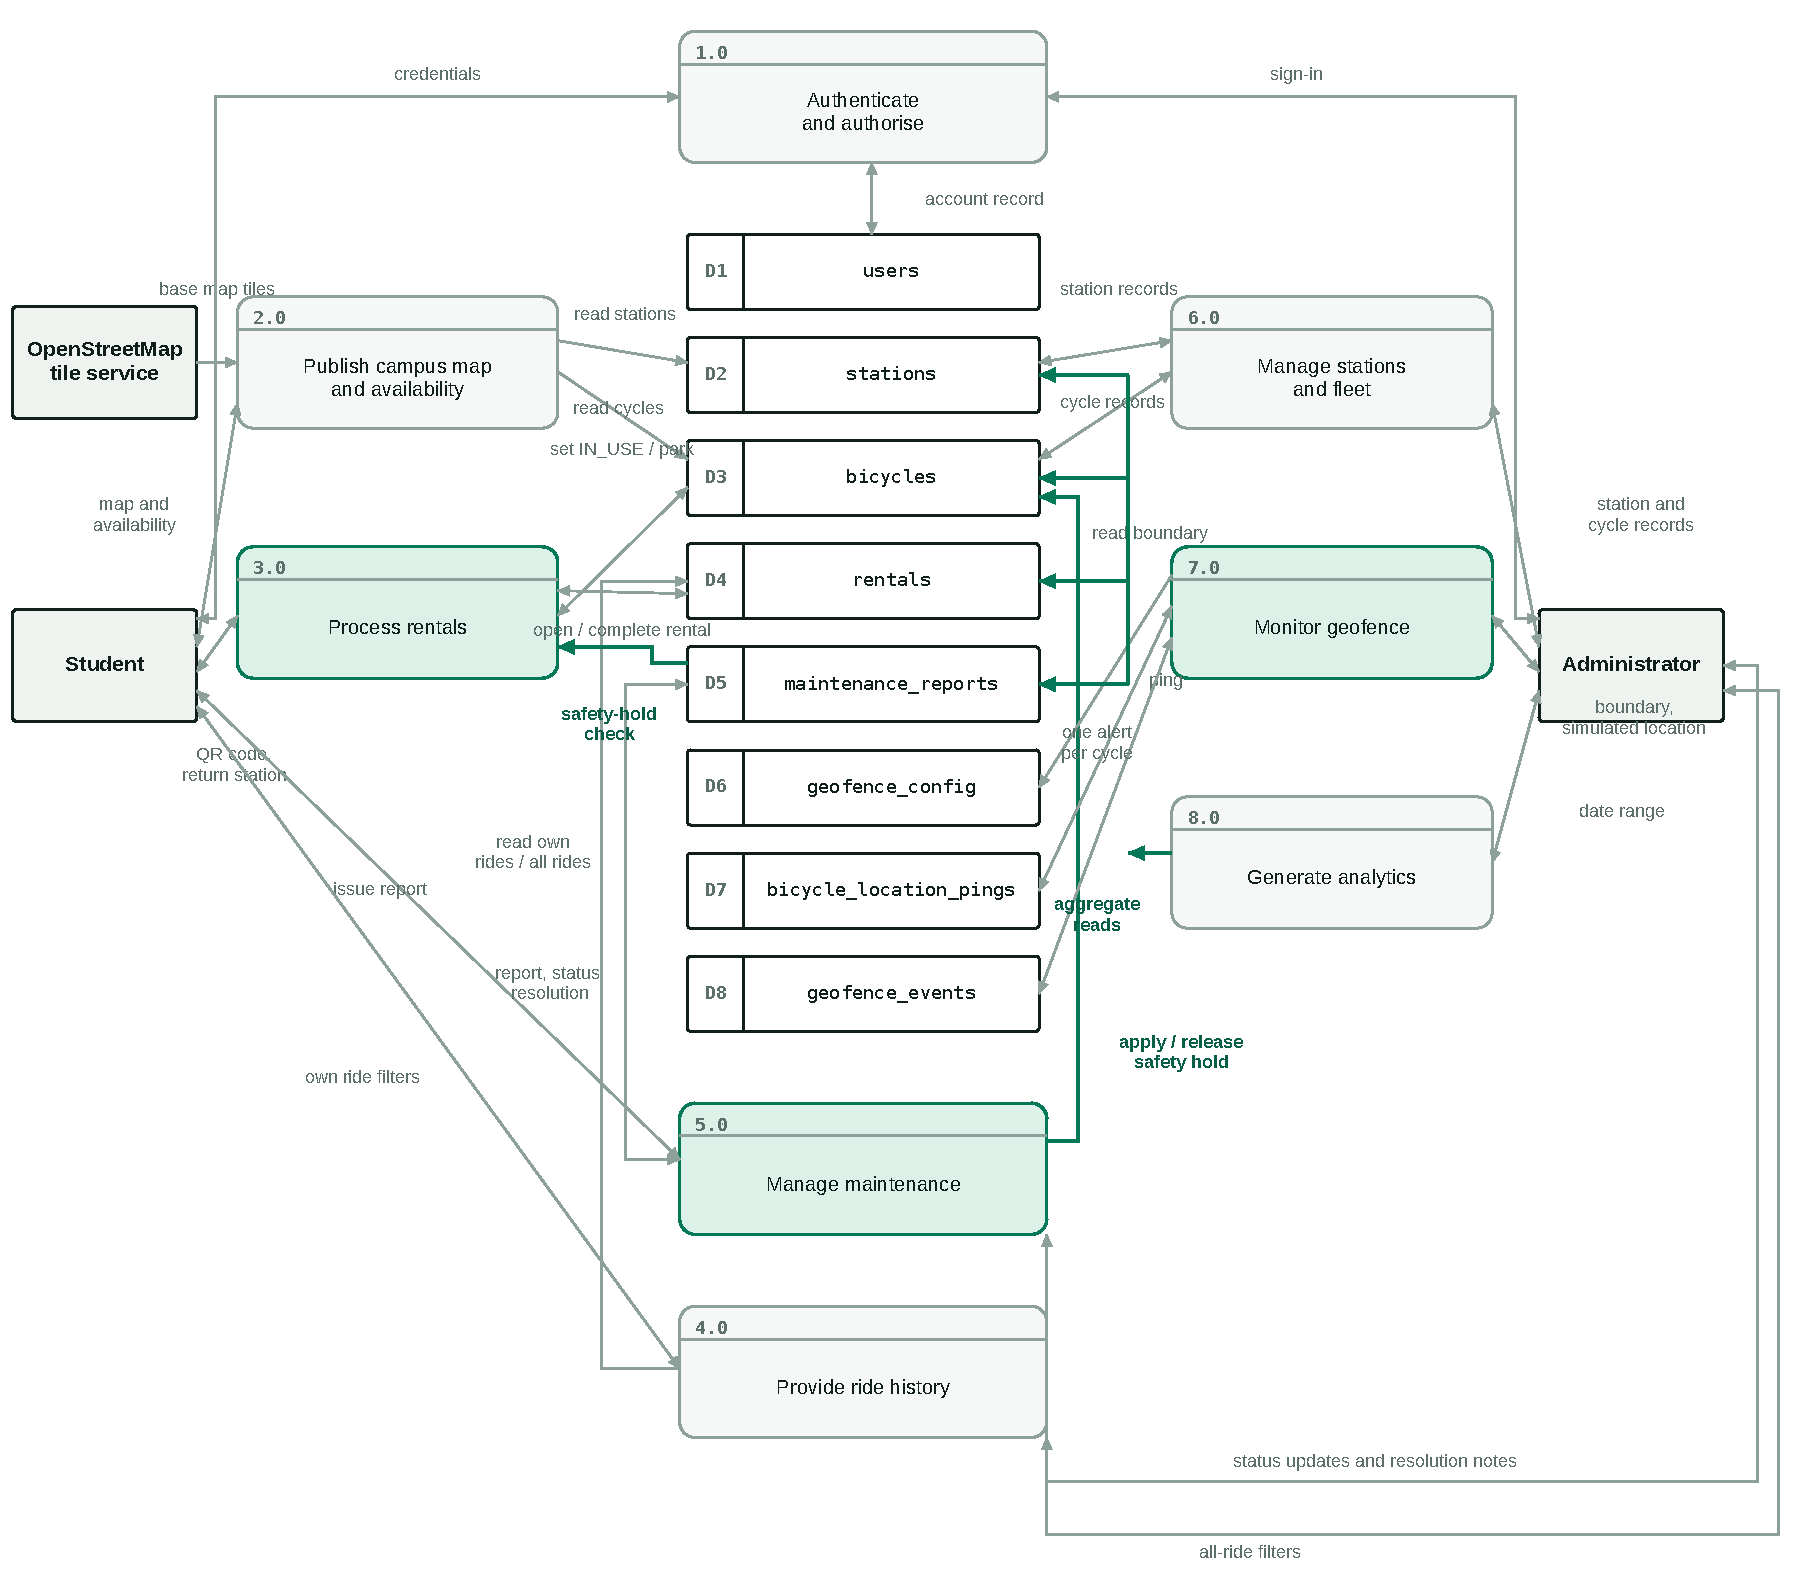
\includegraphics[height=0.85\textwidth]{figures/dfd-l1.pdf}
  \caption{Level-1 data flow diagram. Eight processes
    around the eight tables they use. Writes to a
    store belong to exactly one process; reads cross
    freely.}
  \label{fig:dfd1}
\end{sidewaysfigure}

\section{Database Design}

\subsection{Tables}

The schema is eight tables: four from Phase~1 and four
added by Phase~2 (Table~\ref{tab:schema}). Primary
keys are \texttt{INTEGER GENERATED ALWAYS AS
IDENTITY}, every enumerated column is constrained by a
\texttt{CHECK} that mirrors a constant in the
application code, and an \texttt{updated\_at} trigger
maintains modification timestamps.

\begin{table}[htbp]
\centering
\begin{tabular}{@{}llp{6.1cm}@{}}
\toprule
\textbf{Table} & \textbf{Phase} & \textbf{Contents} \\
\midrule
\texttt{users} & 1 &
  Accounts, bcrypt password hash~\cite{bcrypt}, role \\
\texttt{stations} & 1 &
  Name, location, capacity, status; latitude and
  longitude added in Phase~2 \\
\texttt{bicycles} & 1 &
  Cycle code, QR code, current station, status \\
\texttt{rentals} & 1 &
  Rider, cycle, start and end station, timestamps,
  status \\
\texttt{maintenance\_reports} & 2 &
  Reported fault, severity, lifecycle status,
  reporter, resolution \\
\texttt{geofence\_config} & 2 &
  Campus boundary polygon stored as JSONB \\
\texttt{bicycle\_location\_pings} & 2 &
  Every submitted position, with its source \\
\texttt{geofence\_events} & 2 &
  Boundary violations, de-duplicated per cycle \\
\bottomrule
\end{tabular}
\caption{Database tables.}
\label{tab:schema}
\end{table}

\subsection{Invariants Enforced in the Database}
\label{sec:concurrency}

Rules that must hold under concurrent use are pushed
into the database, because application-level checks of
the form \emph{read, decide, then write} are unsafe
when two requests interleave between the read and the
write~\cite{bernstein1987}. The schema therefore
carries:

\begin{itemize}
  \item \texttt{uq\_active\_rental\_per\_user} and
    \texttt{uq\_active\_rental\_per\_bicycle} ---
    partial unique indexes making a second active
    rental impossible rather than merely unlikely;
  \item \texttt{uq\_geofence\_open\_event\_per\_bicycle}
    --- the same device applied to alerts, which is
    what prevents a cycle left outside the boundary
    from generating an unbounded number of them;
  \item \texttt{uq\_geofence\_single\_active} --- at
    most one active boundary configuration;
  \item \texttt{chk\_ended\_at} and
    \texttt{chk\_maintenance\_resolved} --- a
    completed ride must carry an end timestamp, and a
    resolved report a resolution time;
  \item \texttt{chk\_stations\_coords\_paired} and
    range checks --- a station has both coordinates or
    neither, and each lies within its valid range.
\end{itemize}

Above these, the service layer takes explicit row
locks. Starting a rental, returning one, filing a
report and changing a bicycle's status all run inside
a transaction that holds \texttt{SELECT \ldots{} FOR
UPDATE} on the bicycle row, so those four operations
are serialised against each other for a given cycle.
The database constraints remain as a second line of
defence, and the unique-violation error codes they
raise are translated into readable messages rather
than surfacing as failures.

\subsection{Migrations and Seed Data}
\label{sec:migrations}

Phase~2 could not rebuild the database, because a
Phase~1 instance already held accounts and rental
history. The schema change is therefore delivered as
an additive, idempotent migration: it adds columns and
tables, creates constraints only when they are absent,
and never drops or truncates anything. Running it
twice has the same effect as running it once. A
separate, equally idempotent seed script fills in
station coordinates and installs a campus boundary,
and adds demonstration maintenance reports only when
that table is still empty, so that a database holding
genuine reports is left untouched.

\section{Implementation Details}

\subsection{Authentication and Access Control}

Passwords are hashed with bcrypt~\cite{bcrypt} at a
configurable cost factor; the hash never leaves the
database layer. A successful sign-in returns a JWT
carrying the user id and role, which the browser
attaches to every subsequent request.

Two decisions here are deliberate. First, public
registration always creates a student: there is no
input through which a caller can request the
administrator role, which removes privilege escalation
by construction. Second, and more pervasively,
\textbf{the identity used for authorisation is always
taken from the verified token, never from the request
body or query string}. A request for ride history
carries no user id at all; the server derives it. This
single convention is what makes objective~5 hold
across every endpoint rather than endpoint by
endpoint.

\subsection{Rentals and the Return Workflow}

A rental begins when a student submits a QR code. In
one transaction, the service checks that the student
holds no active ride, locks and loads the bicycle by
its QR code, verifies that it is available and free of
any safety hold, creates the rental, and marks the
bicycle \texttt{IN\_USE} with no station --- a cycle
in use is parked nowhere. The return reverses this:
the ride is completed with an end station and
timestamp, and the bicycle is parked at that station.

Capacity is enforced when an administrator assigns
cycles to a station, but never on return. A student
must always be able to end a ride; refusing a return
because a station is notionally full would strand
them.

\subsection{Campus Map and Station Availability}

Availability is defined once, in a single module, and
every surface that displays it --- the station list,
the station detail page, the map, the student
dashboard --- derives its figures from that one
definition:

\begin{itemize}
  \item \texttt{available\_count}: bicycles with
    status \texttt{AVAILABLE} parked at the station;
  \item \texttt{availability\_pct}:
    \texttt{available\_count} as a percentage of
    capacity, defined as zero when capacity is zero so
    that no screen can divide by zero;
  \item \texttt{availability\_level}: one of
    \texttt{INACTIVE}, \texttt{NONE}, \texttt{LOW} or
    \texttt{GOOD}. A station is \texttt{LOW} when at
    most two cycles remain \emph{or} fewer than 20\%
    of its capacity is available --- the count catches
    a nearly-empty large station, the percentage a
    nearly-empty small one.
\end{itemize}

The map itself is drawn with Leaflet~\cite{leaflet}
over OpenStreetMap tiles~\cite{openstreetmap}
(Figure~\ref{fig:uimap}). Markers are generated from
the station data, so a marker always carries the
current count; the frontend contains no availability
figures of its own. Stations that have no coordinates
are reported explicitly rather than silently omitted.

\begin{figure}[htbp]
  \centering
  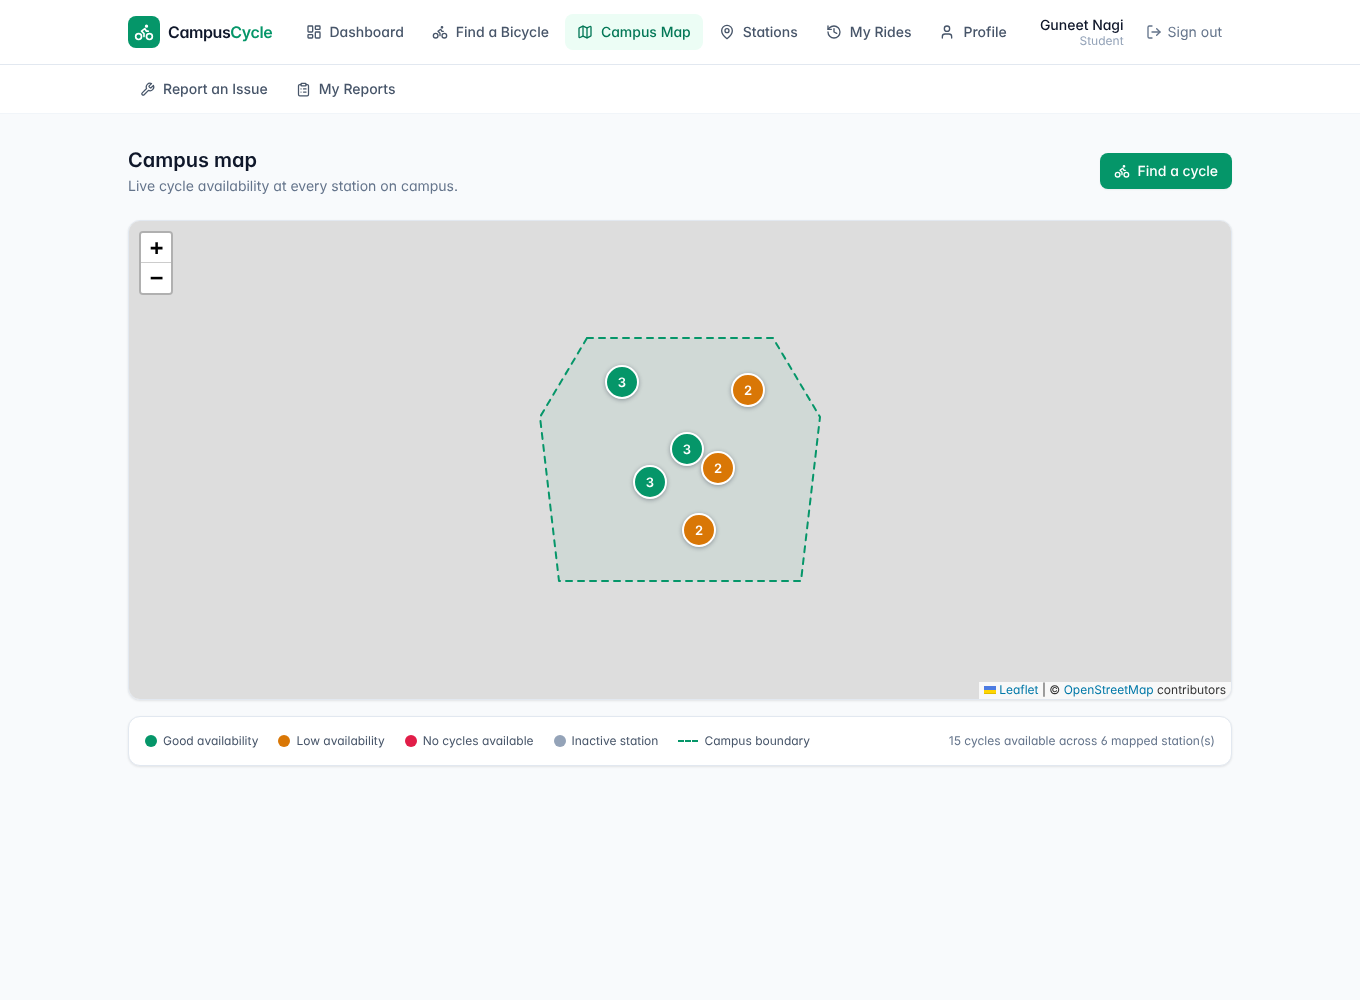
\includegraphics[width=\textwidth]{figures/ui-student-map.png}
  \caption{Student campus map: one marker per station,
    coloured and numbered by live availability, with
    the configured campus boundary drawn as a dashed
    outline. The basemap tiles are fetched from
    OpenStreetMap at run time and are absent in this
    capture, which was taken on a host without
    external network access.}
  \label{fig:uimap}
\end{figure}

\subsection{Ride History}

Ride durations are computed by PostgreSQL from the
stored \texttt{TIMESTAMPTZ} values rather than in the
browser: a completed ride reports
\texttt{ended\_at} $-$ \texttt{started\_at}, an active
one reports \texttt{NOW()} $-$ \texttt{started\_at},
and a ride with a missing or inconsistent timestamp
reports no duration at all rather than a negative or
invented one. Administrators additionally get filters
by date range, cycle, station and status, with
pagination; no endpoint returns an unbounded result
set.

\subsection{Maintenance and the Safety Hold}

This module is the one place where a user-facing
feature and a safety property meet, and
Figure~\ref{fig:dfd2m} shows the resulting flow in
full.

\begin{figure}[htbp]
  \centering
  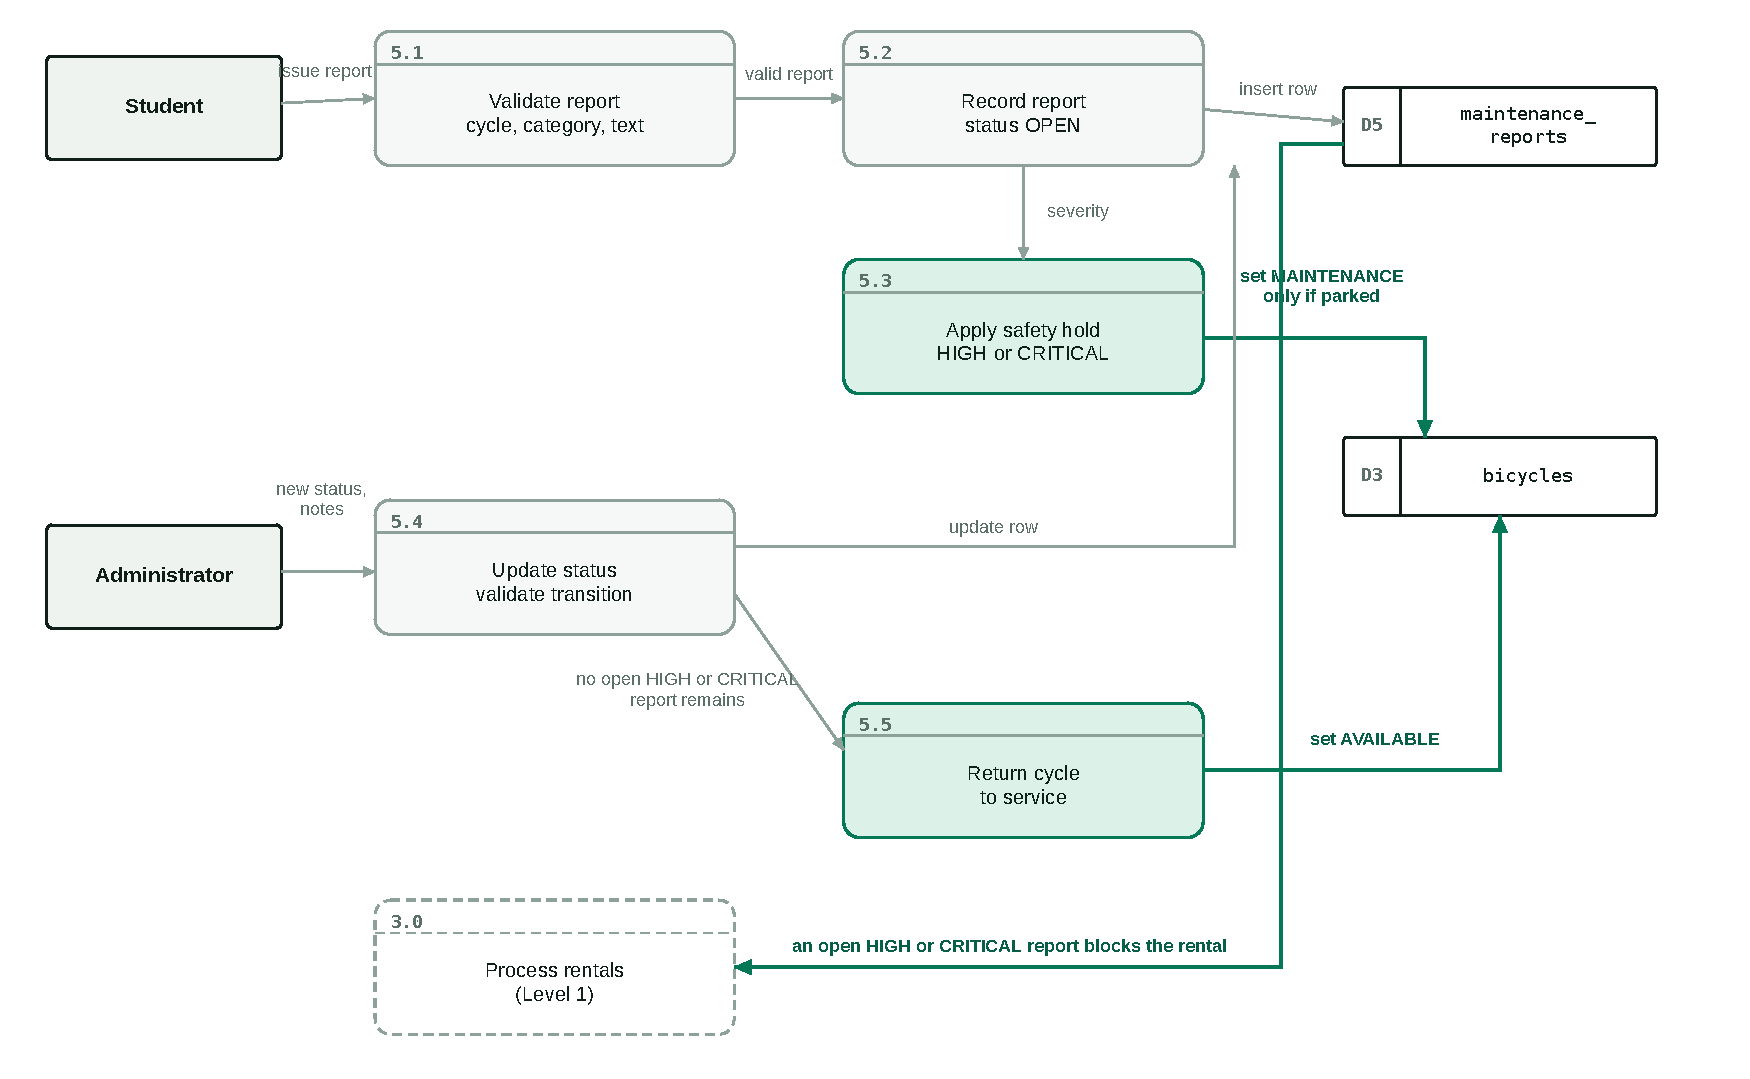
\includegraphics[width=\textwidth]{figures/dfd-l2m.pdf}
  \caption{Maintenance and the safety hold. The
    highlighted path is the invariant: an unresolved
    high-severity report blocks the rental process and
    blocks any return to service.}
  \label{fig:dfd2m}
\end{figure}

A student reports a fault against a cycle with a
category, a description and a severity
(Figure~\ref{fig:uireport}). Severity drives
everything that follows:

\begin{itemize}
  \item A \texttt{HIGH} or \texttt{CRITICAL} report
    places the cycle on a \textbf{safety hold}. If the
    cycle is parked it is moved to
    \texttt{MAINTENANCE} immediately. If it is out on
    a ride the rider is not interrupted --- taking a
    cycle out from under someone mid-ride would be
    worse than the fault --- and the hold is applied
    when it is returned, so it is parked as
    \texttt{MAINTENANCE} rather than
    \texttt{AVAILABLE}.
  \item A \texttt{LOW} or \texttt{MEDIUM} report is
    recorded for review and leaves the cycle in
    service.
\end{itemize}

While a hold exists the cycle cannot be rented, cannot
be parked as available on return, and cannot be forced
back into service by an administrator. All three
routes consult the same check. Reports move through
\texttt{OPEN} $\rightarrow$ \texttt{IN\_PROGRESS}
$\rightarrow$ \texttt{RESOLVED} $\rightarrow$
\texttt{CLOSED}, with reopening permitted from the two
middle states and \texttt{CLOSED} terminal; invalid
transitions are refused, and resolution notes are
required to resolve or close a report
(Figure~\ref{fig:uimaint}).

Resolving a report does \emph{not} by itself return
the cycle to service. Clearing a report is a statement
about a record; returning a cycle to service is a
statement about a physical object that someone must
have actually repaired and parked. The system
therefore requires a separate, explicit administrative
action, and permits it only once no hold remains.

\begin{figure}[htbp]
  \centering
  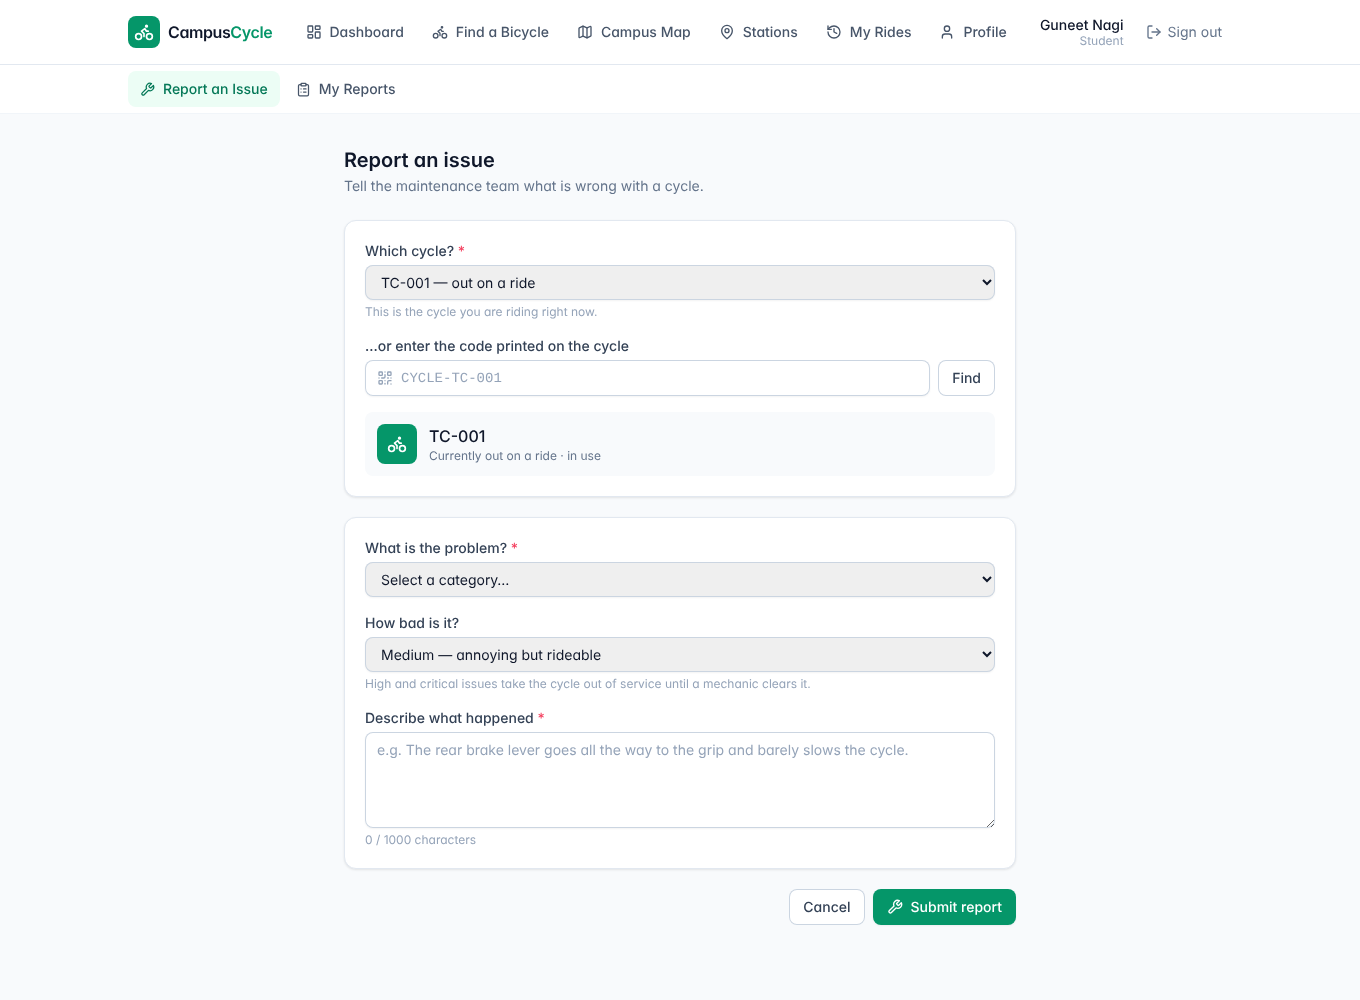
\includegraphics[width=0.86\textwidth]{figures/ui-student-report.png}
  \caption{Fault reporting. The cycle is pre-selected
    from the student's active ride, and the form warns
    that a safety-severity report takes the cycle out
    of service.}
  \label{fig:uireport}
\end{figure}

\begin{figure}[htbp]
  \centering
  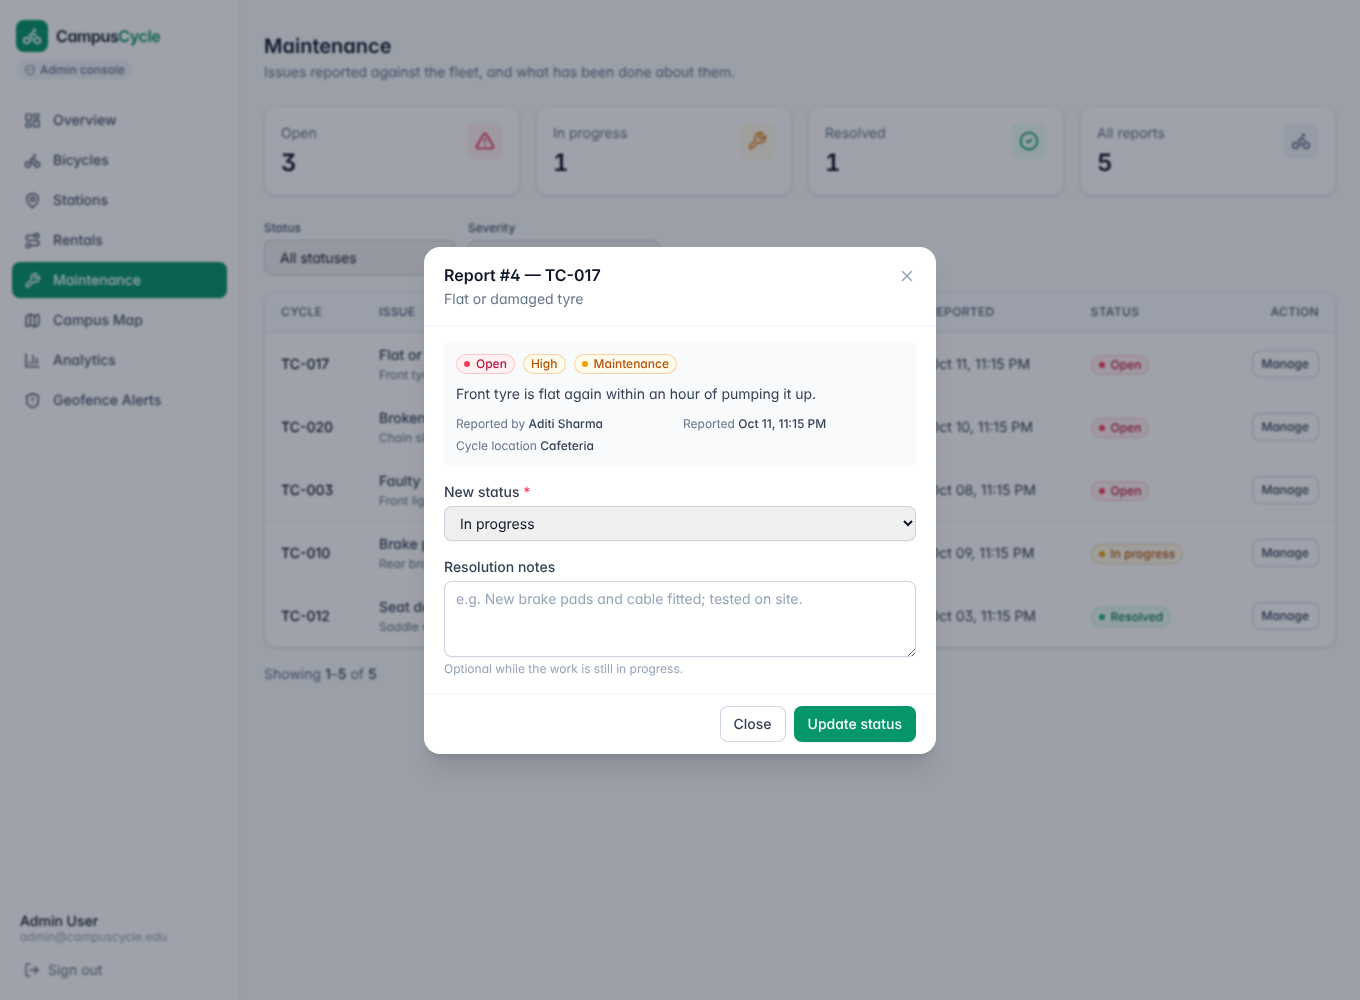
\includegraphics[width=0.86\textwidth]{figures/ui-admin-maintenance-modal.png}
  \caption{Administrative maintenance queue. Only the
    transitions permitted from the report's current
    state are offered.}
  \label{fig:uimaint}
\end{figure}

\subsection{Usage Analytics}

Every figure on the analytics dashboard
(Figure~\ref{fig:uianalytics}) is a PostgreSQL
aggregate over the live tables; nothing is cached or
hard-coded. The page separates two kinds of number
that are easily confused: a \emph{snapshot} of the
fleet together with all-time totals, which the date
filter does not affect, and \emph{period} figures
counting only rides that started inside the selected
range.

Three details were necessary for the figures to be
trustworthy. Empty days are generated with
\texttt{generate\_series} and joined against, so a
quiet week produces zeros on a continuous axis rather
than a gap. Averages over an empty set return no value
rather than zero, which are different statements.
Day and hour buckets are computed in an explicitly
configured reporting timezone, because
\texttt{date\_trunc} otherwise follows the database
session's timezone: during development this placed
rides on the wrong calendar day whenever the server
session ran in UTC while the campus is at UTC$+$05:30.

\begin{figure}[htbp]
  \centering
  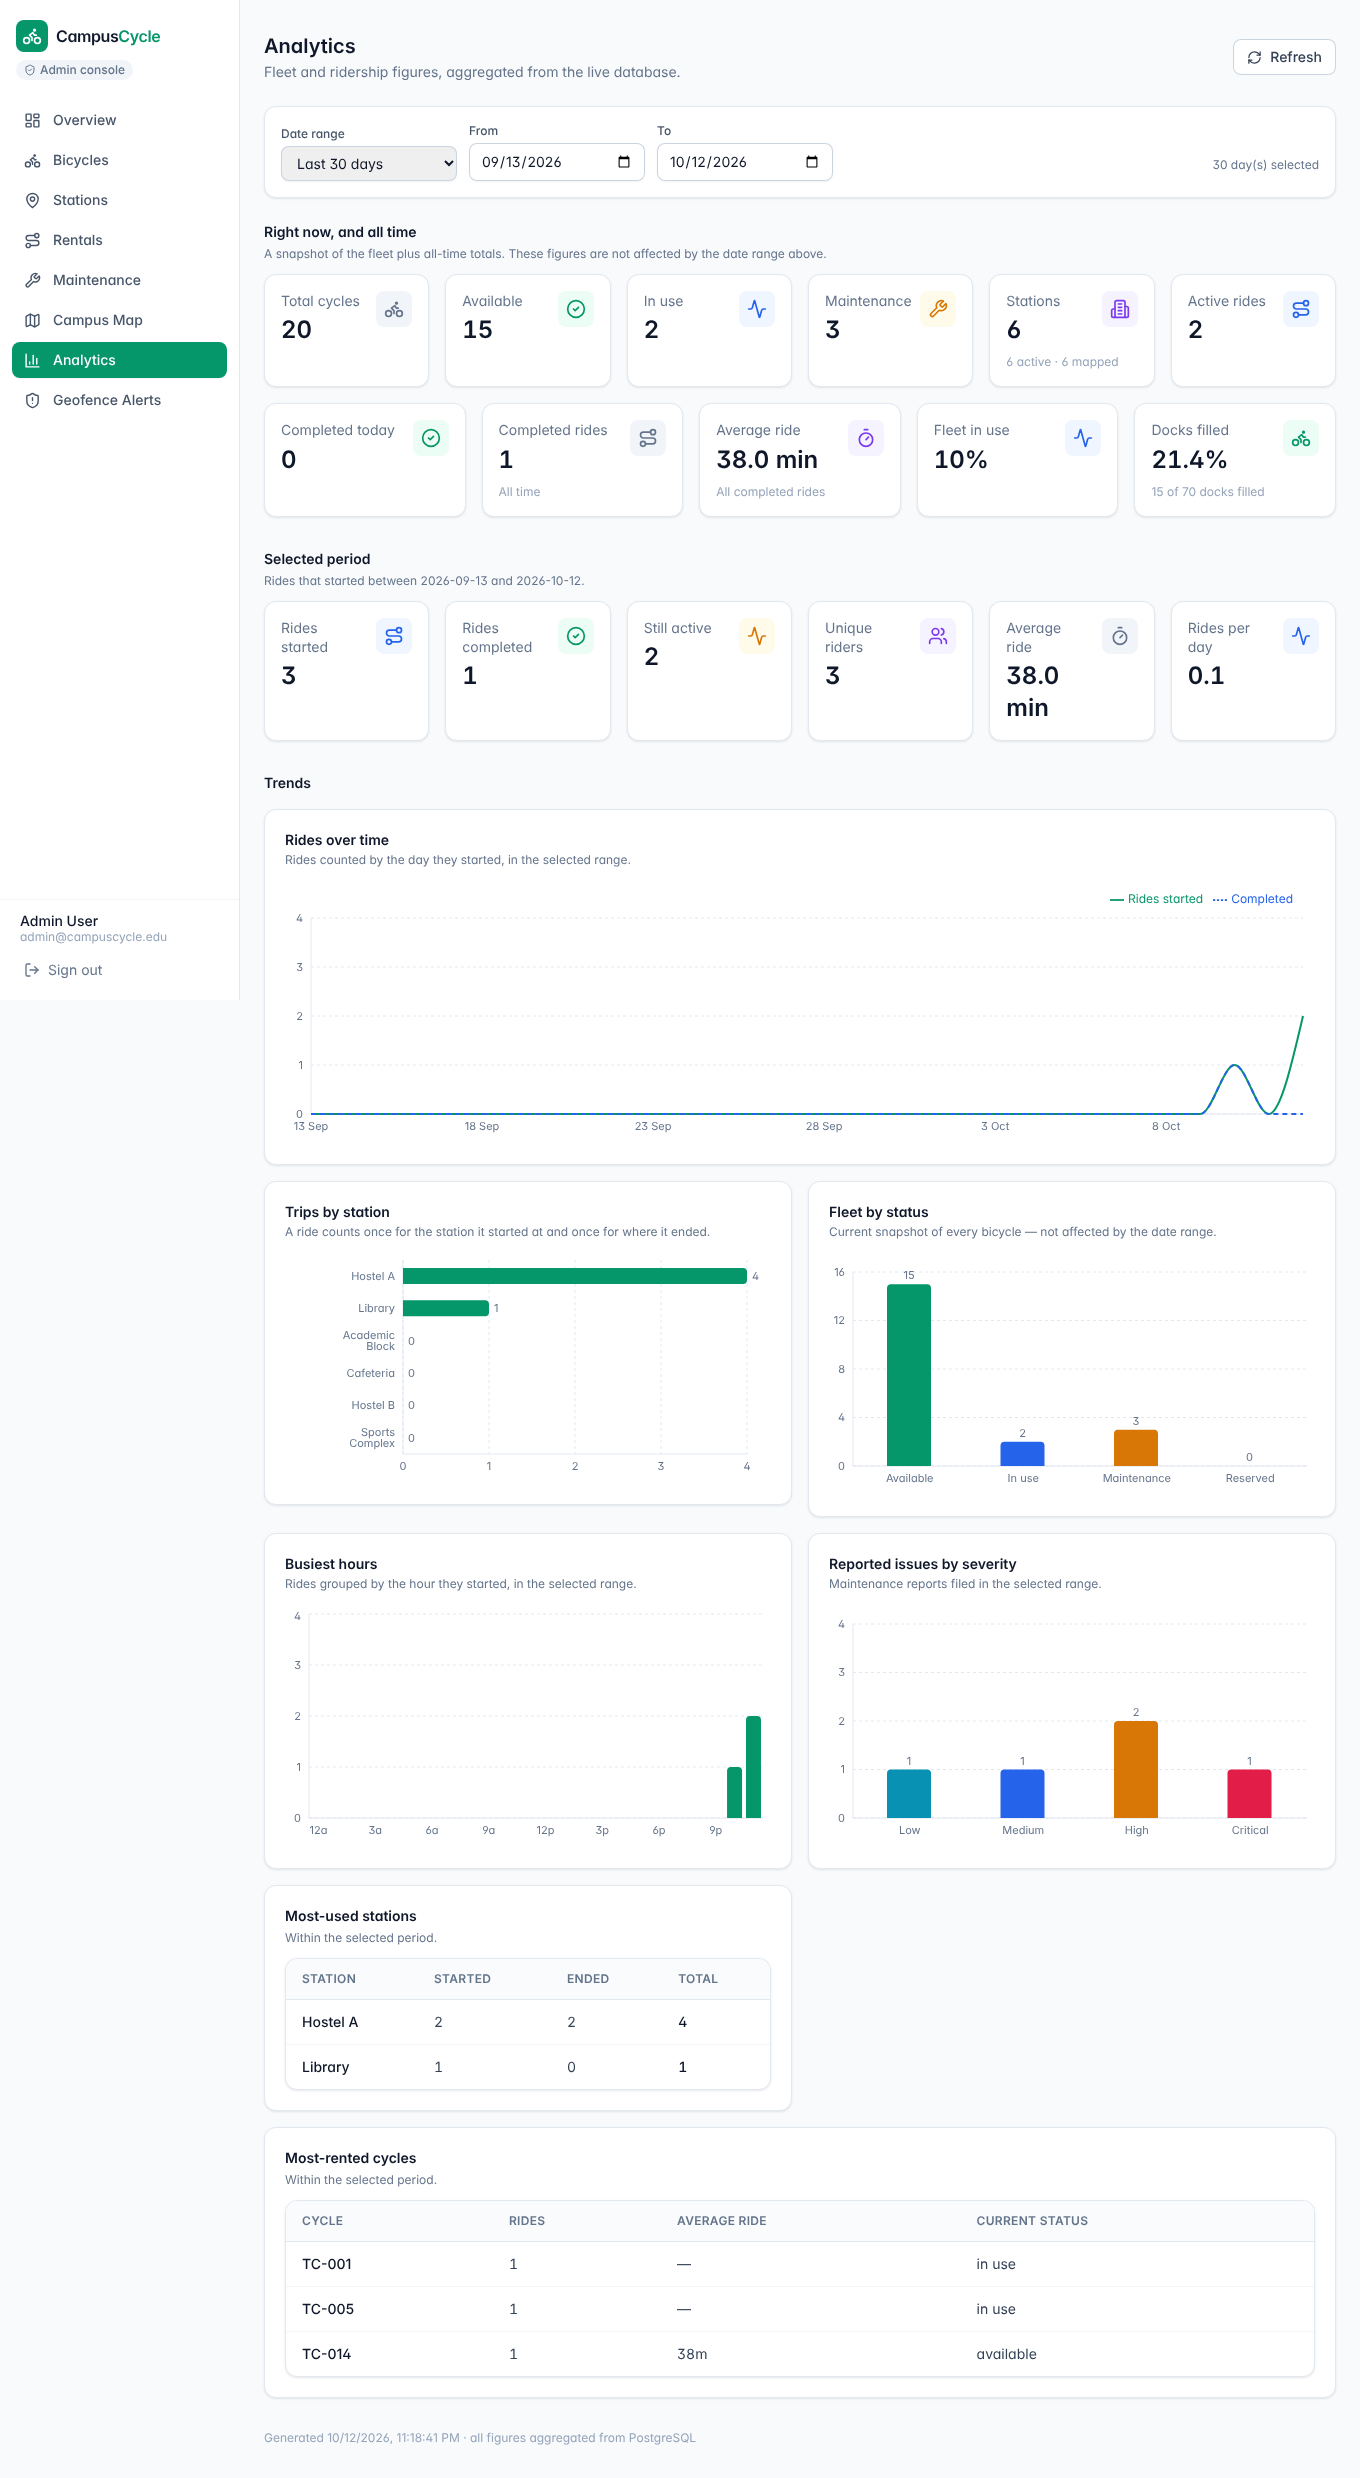
\includegraphics[width=\textwidth]{figures/ui-admin-analytics.png}
  \caption{Analytics dashboard. Snapshot and all-time
    figures are kept visually and textually separate
    from figures for the selected period.}
  \label{fig:uianalytics}
\end{figure}

\subsection{Software-Based Geofencing}
\label{sec:geofence}

\textbf{The bicycles carry no GPS hardware.} There is
no continuous tracking in this system, and the
application does not present one. Every position it
holds was explicitly submitted through an
administrator-only endpoint and is stored with its
source; only simulated positions are accepted, and a
position claiming to come from a device is rejected
until a real integration exists. A student's browser
location is never accepted as a bicycle's position,
which is why the endpoint takes an explicit cycle
identifier and is closed to students.

\begin{figure}[htbp]
  \centering
  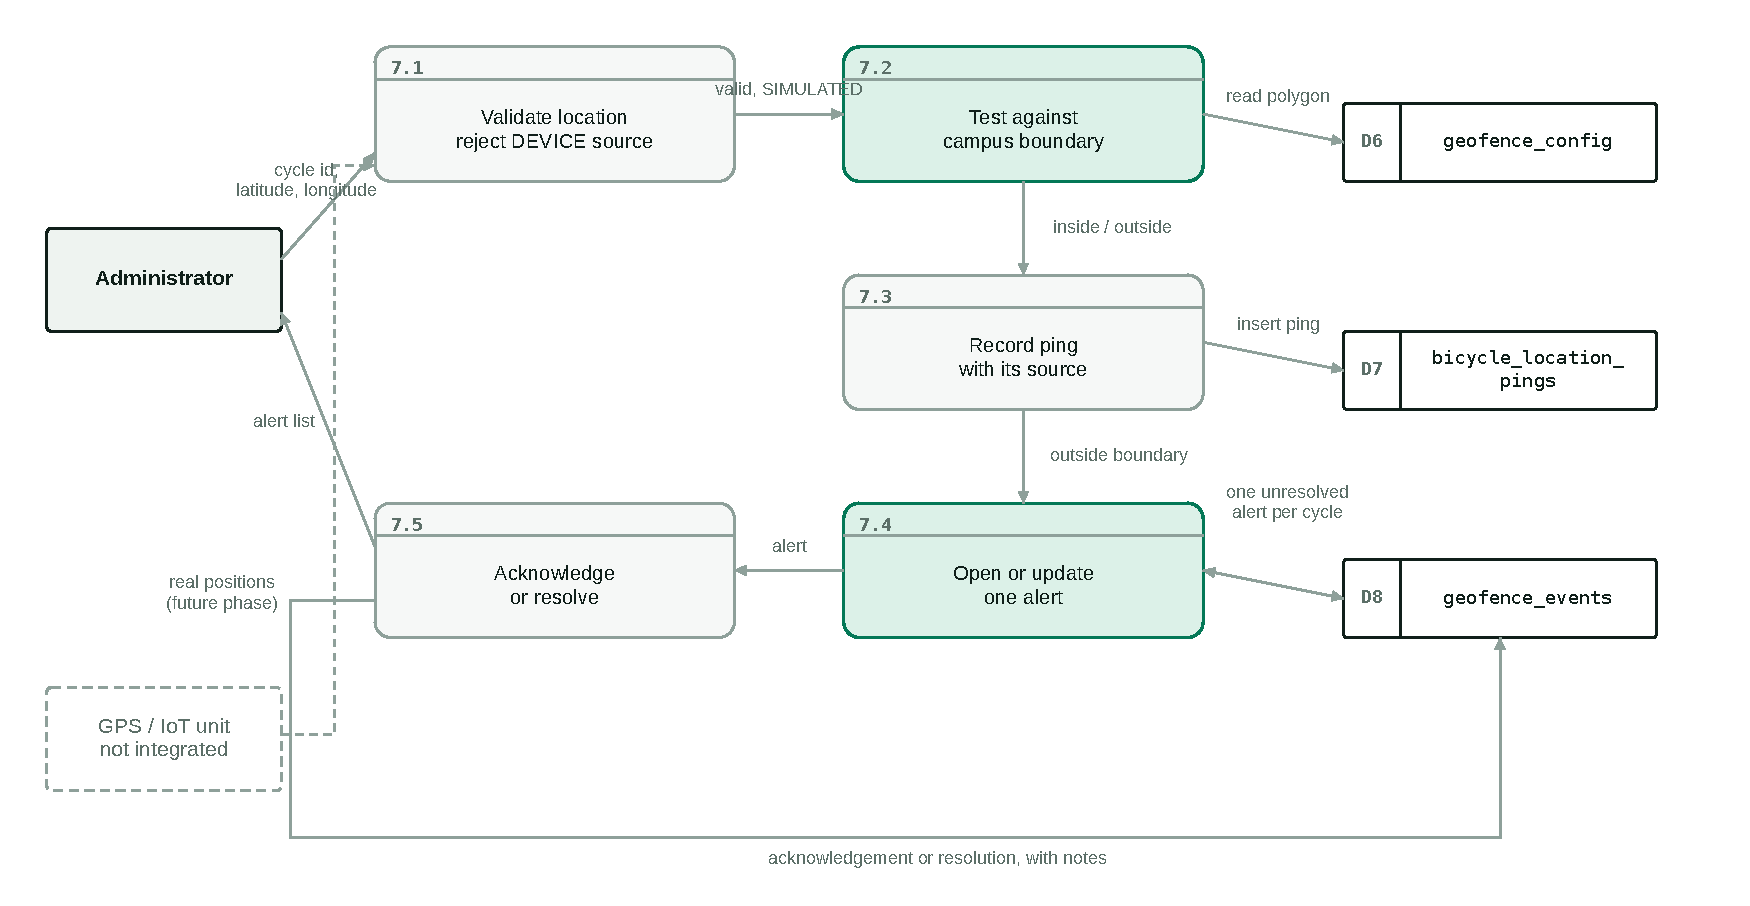
\includegraphics[width=\textwidth]{figures/dfd-l2g.pdf}
  \caption{Geofencing. The source is validated before
    anything else, and one unresolved alert per cycle
    is what keeps a wandering bicycle from flooding
    the alert list.}
  \label{fig:dfd2g}
\end{figure}

The campus boundary is a configurable polygon stored
as JSONB and tested with a ray-casting
point-in-polygon algorithm~\cite{shamos1976}; at the
scale of one campus, treating latitude and longitude
as a plane introduces no meaningful error. A position
outside the boundary opens an alert recording the
cycle, the time, the coordinates and the ride in
progress. A \emph{repeated} breach does not open
another: it increments the existing alert's counter
and updates its last known position, a rule enforced
by the partial unique index named earlier. A cycle
seen back inside records that fact but does not close
the alert, because whether the situation is resolved
is a judgement for a person
(Figure~\ref{fig:uigeofence}).

\begin{figure}[htbp]
  \centering
  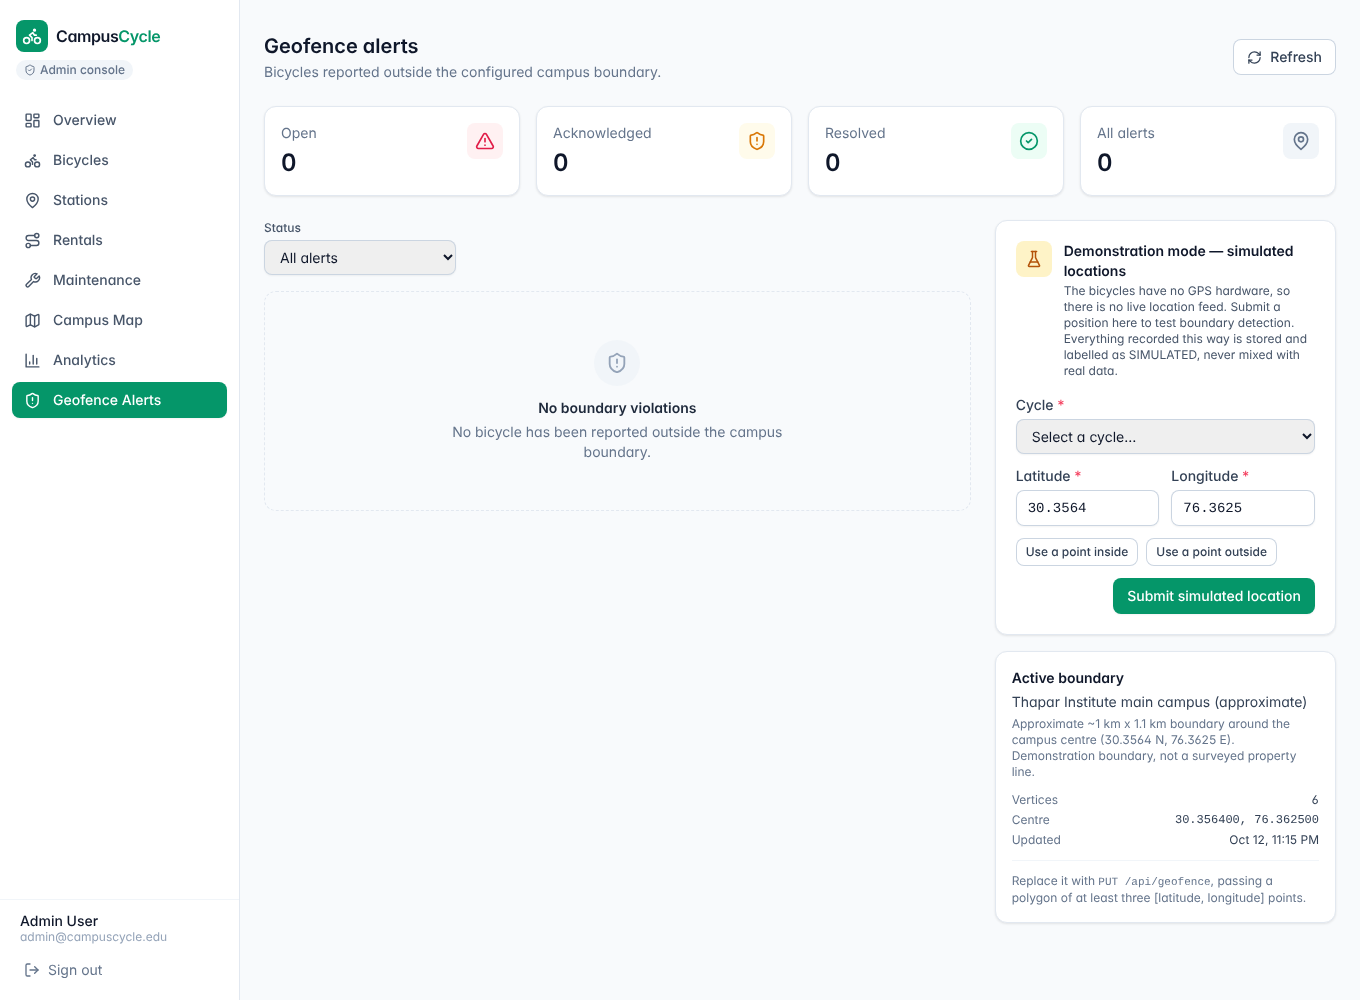
\includegraphics[width=\textwidth]{figures/ui-admin-geofence.png}
  \caption{Geofence alerts, with the clearly labelled
    demonstration panel used to submit simulated
    positions.}
  \label{fig:uigeofence}
\end{figure}

\section{Security Considerations}

\begin{itemize}
  \item \textbf{Credentials.} Passwords are stored
    only as bcrypt hashes. Sign-in failures return one
    uniform message, so the response cannot be used to
    discover which email addresses are registered.
  \item \textbf{Authorisation.} Role checks sit in
    middleware on the route, not in the handler, so an
    endpoint cannot be added without a decision about
    who may reach it.
  \item \textbf{Injection.} Every query is
    parameterised; no SQL is assembled from user
    input.
  \item \textbf{Secrets.} The JWT secret and database
    credentials are read from the environment, and the
    environment file is excluded from version control.
    A test asserts that no password hash, token secret
    or connection string appears in any API response.
  \item \textbf{Transport and headers.} \texttt{helmet}
    sets standard security headers and CORS is
    restricted to the configured origin.
\end{itemize}

% ===== CHAPTER 3: RESULTS & EVALUATION =====

\chapter{Results and Evaluation}

\section{Testing Methodology}

Testing is automated and runs against a real
PostgreSQL database rather than a mocked one, because
most of the properties worth testing in this system
--- uniqueness under concurrency, transactional
consistency, the correctness of aggregate queries ---
exist only in the database and would be assumed away
by a mock.

\begin{itemize}
  \item \textbf{Integration and end-to-end testing.}
    Two suites rebuild the schema, apply the
    migrations, load the seed data, start the Express
    application on an ephemeral port and drive it over
    real HTTP. They cover the full rental lifecycle,
    role-based access control, the maintenance and
    safety-hold workflow, analytics figures checked
    against direct SQL counts, and geofence detection
    and de-duplication.
  \item \textbf{Concurrency testing.} Two sign-ins
    issue simultaneous requests for the same bicycle;
    the suite asserts that exactly one succeeds and
    one is refused.
  \item \textbf{Regression testing.} The Phase~1 suite
    is run unchanged after every Phase~2 change. Its
    one modification was to apply the new migrations
    before seeding; no assertion was altered or
    removed.
  \item \textbf{User-interface testing.} A browser
    test drives the real interface end to end: a
    student files a critical fault report, the cycle
    disappears from the list of rentable cycles, an
    administrator resolves the report and is offered
    the return-to-service action, then simulates a
    boundary breach and confirms that repeating it
    produces no second alert.
  \item \textbf{Build verification.} The production
    frontend build is run as part of the check, so a
    broken import or unused dependency fails
    immediately.
\end{itemize}

\section{Results}

\begin{table}[htbp]
\centering
\begin{tabular}{@{}lrrl@{}}
\toprule
\textbf{Suite} & \textbf{Checks} & \textbf{Passed} &
\textbf{Covers} \\
\midrule
Phase~1 end-to-end   & 25  & 25  & Rental lifecycle,
  RBAC, concurrency \\
Phase~2 end-to-end   & 139 & 139 & Map, history,
  maintenance, analytics, \\
                     &     &     & geofencing, access
  control \\
Browser flow         & 17  & 17  & Student and
  administrator journeys \\
\midrule
\textbf{Total}       & \textbf{181} & \textbf{181} & \\
\bottomrule
\end{tabular}
\caption{Automated test results. All suites pass with
  no failures.}
\label{tab:tests}
\end{table}

A selection of the properties asserted, chosen because
each corresponds to an objective rather than to a
screen:

\begin{itemize}
  \item Two students requesting the same bicycle
    simultaneously produce exactly one rental and one
    refusal.
  \item A seeded 38-minute ride reports a duration of
    exactly 2280 seconds; a ride still in progress
    reports a duration that advances.
  \item A student requesting another student's ride
    receives 403; an unknown ride identifier receives
    404; a malformed one receives 400.
  \item A cycle with an unresolved critical report
    cannot be rented, and an administrator attempting
    to mark it available receives 409.
  \item Three successive out-of-bounds positions
    produce one alert with a count of three, not three
    alerts.
  \item Every administrative endpoint returns 403 for
    a student token and 401 for no token.
  \item No password hash, token secret or connection
    string appears in any API response.
\end{itemize}

\section{Scale of the Implementation}

\begin{table}[htbp]
\centering
\begin{tabular}{@{}lr@{}}
\toprule
\textbf{Measure} & \textbf{Value} \\
\midrule
Backend source files            & 53 \\
Backend lines of code           & 5{,}438 \\
Frontend source files           & 64 \\
Frontend lines of code          & 7{,}528 \\
SQL (schema, migration, seeds)  & 551 \\
REST endpoints                  & 44 \\
Database tables                 & 8 \\
Indexes and unique constraints  & 20 \\
Automated checks                & 181 \\
\bottomrule
\end{tabular}
\caption{Implementation size at this evaluation.}
\label{tab:size}
\end{table}

\section{Analysis}

\subsection{Were the Objectives Met?}

Eight of the nine objectives are complete and
evidenced by the tests listed above. The ninth,
demand prediction, was deliberately deferred for the
reason given in Section~\ref{sec:scope}.

One objective deserves a qualified answer. The
geofencing objective is met as specified --- a
boundary is configurable, violations are detected,
recorded, de-duplicated and actionable --- but it
operates on submitted positions rather than measured
ones, because the project has no GPS hardware. Rather
than let the interface imply a tracking capability
that does not exist, the limitation is made explicit
in the API, in the stored data and on screen. The
software is structured so that the eventual hardware
feed replaces one validated input path and nothing
else.

\subsection{Challenges and Their Resolution}

\paragraph{Concurrent access to a single bicycle.}
The first implementation checked a bicycle's
availability and then created the rental, which is
correct when tested by one person and wrong under
load: two requests can both pass the check before
either writes. The resolution was to stop treating
this as application logic. The bicycle row is locked
for the duration of the transaction, and a partial
unique index makes a second active rental impossible
even if the lock were somehow bypassed. The
concurrency test exists to prove the fix rather than
to illustrate the feature.

\paragraph{Keeping a safety rule true everywhere.}
A bicycle can become available through three
different paths: an administrator sets its status, a
ride ends, or it is created. An early version checked
for unresolved faults only in the first. The
resolution was to make the safety hold a single
function consulted by all three paths, and to express
it as a property of the maintenance records rather
than as an extra column on the bicycle --- a flag
would have been one more piece of state capable of
disagreeing with the reports it summarises.

\paragraph{Timezone-dependent analytics.} Rides were
being attributed to the wrong calendar day. The cause
was that day boundaries were computed in Node using
the machine's local timezone while PostgreSQL grouped
them using the database session's timezone. The
resolution was to make the reporting timezone an
explicit configuration value used on both sides, so
that ``today'' means one thing throughout the system.

\paragraph{Migrating a database already in use.} The
schema had to change without discarding Phase~1 data.
The resolution was to separate the destructive
development path from the additive production path:
the base schema remains re-runnable for a fresh
install, while the Phase~2 migration adds only what is
missing and can be run repeatedly without effect.

% ===== CHAPTER 4: CONCLUSION =====

\chapter{Conclusion}

\section{Summary of Work}

CampusCycle is a working campus bicycle-sharing
system. Students sign in, find an available cycle on a
live map or in a filtered list, identify it by its QR
code, ride it between stations, return it, review
their ride history and report faults. Administrators
manage stations and the fleet, inspect every ride,
work reported faults through a maintenance lifecycle,
read usage analytics computed from the live database
and act on geofence alerts.

Across two phases the system comprises 44 REST
endpoints over eight PostgreSQL tables, with 181
automated checks passing against a real database.
Phase~2 was delivered without modifying a single
Phase~1 assertion and without rebuilding the Phase~1
database.

\section{Key Findings}

\begin{itemize}
  \item \textbf{Invariants belong in the database.}
    Every rule that had to survive concurrent use ---
    one active ride per student, one per cycle, one
    unresolved alert per bicycle --- is enforced by a
    partial unique index. Application code states the
    rule clearly and produces a readable error; the
    database guarantees it.

  \item \textbf{A rule enforced in one place is a rule;
    enforced in three, it is a coincidence.} The
    safety hold became reliable only once every path
    that could make a bicycle available consulted the
    same check. The same applies to availability: one
    definition is why the map and the station list
    cannot disagree.

  \item \textbf{Authorisation must not be derived from
    the request.} Taking the user's identity from the
    verified token rather than from a request
    parameter makes ``a student sees only their own
    rides'' a property of the system rather than a
    property of each endpoint.

  \item \textbf{An honest limitation is cheaper than a
    convincing one.} Labelling simulated positions as
    simulated, at every layer, cost a column and a
    validation rule. It leaves the system extensible
    to real hardware and prevents an operator from
    ever mistaking a demonstration for evidence.
\end{itemize}

\section{Limitations}

\begin{itemize}
  \item There is no real-time tracking; bicycle
    positions are administrator-submitted and
    simulated.
  \item There is no demand prediction or
    redistribution advice; that is the next phase.
  \item Rides are free. No pricing, wallet or payment
    integration exists.
  \item The map requires internet access for
    OpenStreetMap tiles; without it, markers and the
    boundary still render over a blank background.
  \item Station coordinates place the demonstration
    stations within the campus but are approximate
    rather than surveyed, and the boundary polygon
    approximates the campus extent rather than the
    legal property line.
  \item There is no password-reset or email
    verification flow.
\end{itemize}

\section{Future Work and Recommendations}

\begin{enumerate}
  \item \textbf{Demand prediction.} Train a regression
    or tree-based model on the recorded rental history
    using station, hour of day, day of week and recent
    demand as features. The analytics layer already
    produces these aggregates, so the model consumes a
    stable schema rather than ad-hoc extraction.

  \item \textbf{Redistribution advice.} Compare
    predicted demand against current station
    occupancy and recommend movements. This requires
    no new data, only the model from the previous
    item.

  \item \textbf{GPS and IoT integration.} Fit tracking
    units and allow device-sourced positions. The
    ingestion path, the storage, the boundary test and
    the alerting already exist; the change is to admit
    a second value in the source column and to accept
    authenticated device traffic.

  \item \textbf{Electronic locks.} With trusted
    hardware the QR workflow could unlock a physical
    lock, closing the gap between a rental record and
    physical possession of the cycle.

  \item \textbf{Payments and membership.} Semester
    passes, penalties for late returns and receipts,
    should the service move beyond free use.

  \item \textbf{Deployment hardening.} Refresh tokens
    with rotation, rate limiting on authentication,
    structured logging, automated backups and a
    continuous integration pipeline running the
    existing suites on every push.
\end{enumerate}

\section{Final Remarks}

The most useful lesson from this project was about
where correctness lives. The features that were
straightforward to build were the ones that are
visible: a form, a list, a chart. The ones that took
real design effort were invisible when working and
only noticeable when broken --- two students must not
get the same bicycle, a cycle reported unsafe must not
reappear as available, a student must not see another
student's rides. Each of these was first written as
application logic, and each became reliable only once
it was pushed down to a single enforcement point,
usually a database constraint, with the application
code reduced to stating the rule clearly and
explaining the refusal.

The second lesson concerns honesty in engineering. It
would have been easy to present the geofencing module
as bicycle tracking, since the screens would look
identical. Recording the provenance of every position
and refusing to accept a simulated one as real cost
very little and leaves both the system and its
documentation truthful about what has actually been
built --- which is also what makes the hardware phase
a straightforward extension rather than a correction.

% ===== BIBLIOGRAPHY =====

% Print bibliography with heading in TOC
\printbibliography[heading=bibintoc]

\end{document}
